\section{Implementation and Evaluation} \label{sec:evaluation}
We implement \sysname as a fork of Mysticeti~\cite{mysticeti} and evaluate it on a geo-distributed AWS testbed. We use the same setup as the Mysticeti paper~\cite{mysticeti}\footnote{
    13 different AWS regions; \texttt{m5.8xlarge} instances (with 32 vCPUs, 128GB RAM, and 10Gbps network); 512 bytes transactions; each data point is the average latency and error bar represent one stdev; benchmarks run for multiple minutes under fixed load.
} and only test for loads up to 50k tx/s to limit costs. We set $t_a = 10\%$ (\Cref{sec:model}) and auxiliary validators propose blocks every few seconds.
We use the notation M-$X$ to indicate Mysticeti running with $X$ validators, and \sysname-$X$-$Y$ to indicate \sysname running with $X$ core validators and $Y$ auxiliary validators.

\begin{figure}[t]
    \vskip -1em
    \centering
    \begin{minipage}{.49\textwidth}
        \centering
        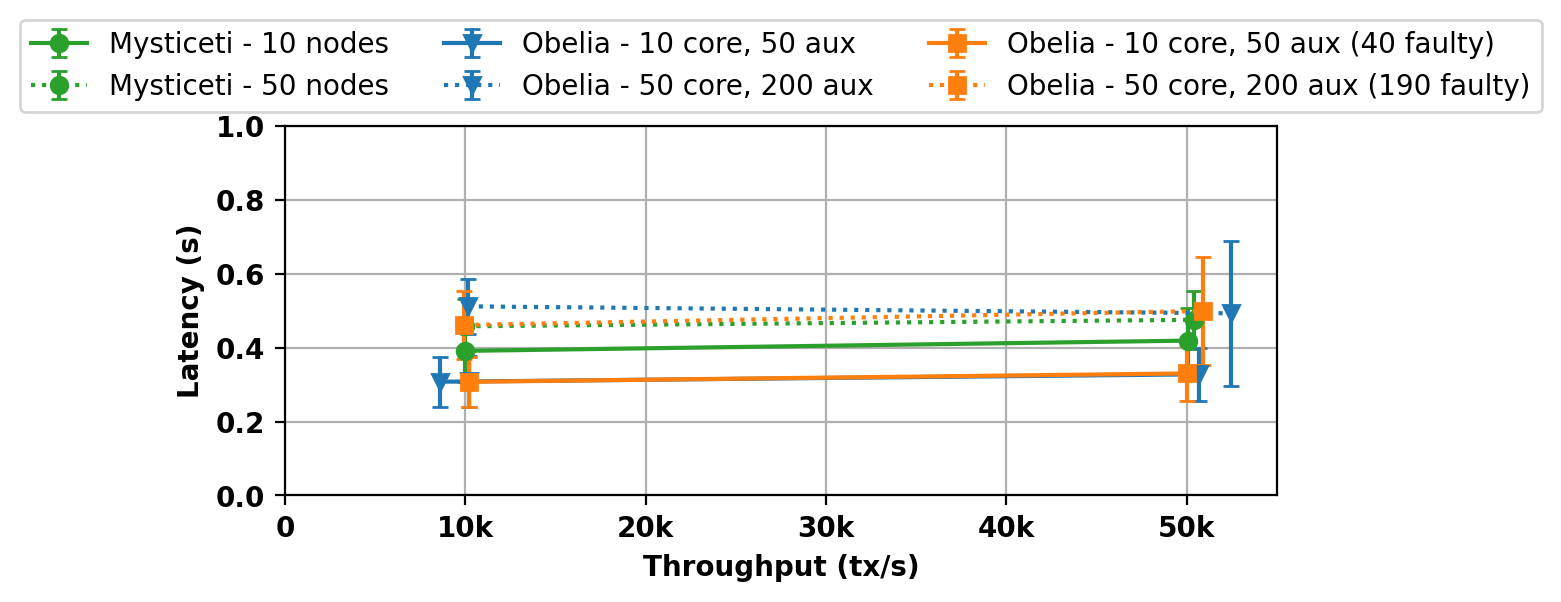
\includegraphics[width=\textwidth]{data/plots/overhead}
    \end{minipage}
    \begin{minipage}{0.48\textwidth}
        \centering
        \vfill
        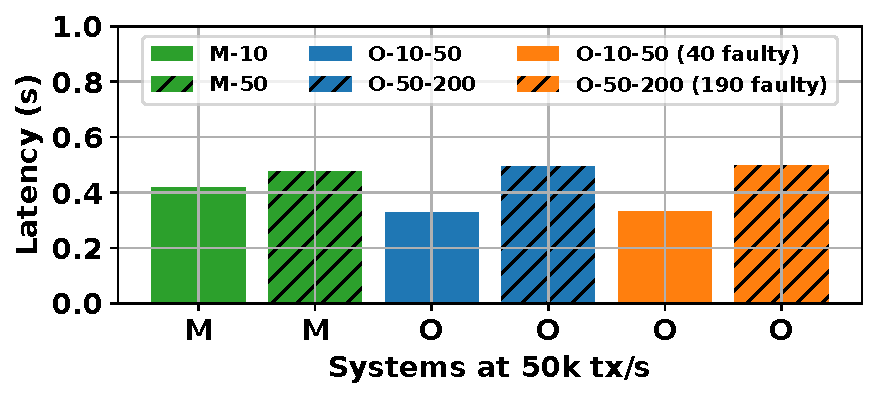
\includegraphics[width=\textwidth]{data/plots/histogram}
    \end{minipage}
    \caption{
        Comparative evaluation of Mysticeti (10 and 50 validators) and \sysname (10 core + 50 auxiliary validators, 50 core + 200 auxiliary validators). Left: throughput-latency graph. Right: Latency zoom at 50k tx/s.
    }
    \label{fig:evaluation}
    \vskip -1em
\end{figure}

\Cref{fig:evaluation} shows that all system configurations maintain a latency of approximately 400ms when processing loads of either 10k tx/s or 50 tx/s. Notably, regardless of the committee size, there is no statistical difference between Mysticeti in its barebone configuration and when equipped with \sysname, confirming our claim \textbf{G4} (from \Cref{sec:goals}) that \sysname introduces negligible overhead. Additionally, \Cref{fig:evaluation} demonstrates that \sysname can scale to 200 auxiliary validators, thus validating our scalability claim \textbf{G5}. Lastly, \Cref{fig:evaluation} (orange lines) illustrates that even a large number of crashed auxiliary validators do not noticeably impact protocol performance, supporting our claim \textbf{G6}.